\documentclass{alex_hü}

\name{Alexander Helbok}
\course{PS Physik}
\hwnumber{10}


\begin{document}
\renewcommand{\labelenumi}{(\alph{enumi})}


\begin{mybox}{1. Selbstinduktion}
	\centering \( U = 50 \unit{V};\quad U_z = 80 \unit{V};\quad R_1 = 1500 \unit{\ohm};\quad I_0 = 0.15 \unit{A};\quad \delta t = 1 \unit{ms} \)
	\tcblower
	\begin{enumerate}
		\item \(  \)
		\begin{minipage}{\textwidth}
			\hspace{2cm}
			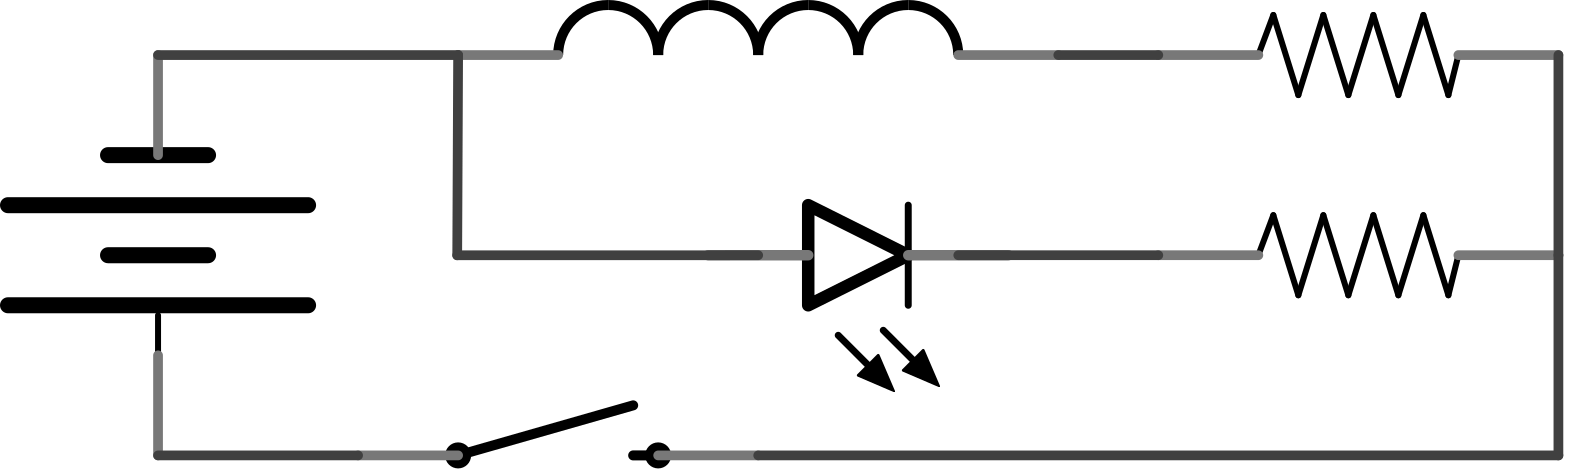
\includegraphics[scale=2]{Ind.png}
		\end{minipage}\vspace{0.5cm}
	\tcbline
		\item \( R2 = \tfrac{U}{I_0};\quad U_{\text{ind}} = U(R_1 + R_2)\)
		\begin{flalign*}
			L\dv{I}{t} &= -I(R_1 + R_2) &&\\
			I(t) &= I_0\, \mathrm{e}^{\supfrac[-]{R_1 + R_2}{L}t} &&\\
			U(t) &= -L\dv{I(t)}{t} = I_0(R_1 + R_2)\, \mathrm{e}^{\supfrac[-]{R_1 + R_2}{L}t} &&\\ 
			U(10^{-6}) &= 80 \quad \Rightarrow \quad L = \dl{1.48 * 10^{-3} \unit{H}} &&
		\end{flalign*}
	\tcbline
		\item \(  \)
		\begin{flalign*}
			U + L\dv{I}{t} &= -IR_2 &&\\
			I(t) &= I_0\left(1 - \mathrm{e}^{\supfrac[-]{R_2}{L}t}\right) &&\\
			I(t)/I_0 &= 0.99 \quad \Rightarrow \quad t = \dl{2.05 * 10^{-5} \unit{s}} &&
		\end{flalign*}
	\tcbline
		\item 
			The Diode is current blocking in one direction and permissive in the other. When the circuit is closed current flows in the wrong direction, whereas when the circuit is opened current flows from the Inductor ind the permissive direction to the diode.
	\end{enumerate}
\end{mybox}

\begin{mybox}{2. Transformator}
	\centering \( U_1 = 230 \unit{V} \)
	\tcblower
	\begin{enumerate}
		\item \(  \)
		\begin{flalign*}
			U_2 &= \dl{U_1\tfrac{N_2}{N_1}} &&
		\end{flalign*}
	\tcbline
		\item \( N_2 = 1;\quad R_2 = 0.2 \unit{\ohm};\quad P = 800 \unit{W} \)
		\begin{flalign*}
			P &= \tfrac{U_2^2}{R_2} &&\\
			U_2 &= \sqrt{PR_2} &&\\
			N_1 &= \tfrac{U_1N_2}{\sqrt{PR_2}} = \dl{18.18} &&
		\end{flalign*}
	\tcbline
		\item \(  \)
		\begin{flalign*}
			I &= \tfrac{P}{U} = \dl{3.48 \unit{A}} &&
		\end{flalign*}
	\tcbline
		\item 
		Without using a spool on the underside of the pots ($\Rightarrow N = 1$) you have to use a lot of current to heat the pot. That's why heating via induction utilizes eddy currents to heat more efficiently.
	\end{enumerate}
\end{mybox}

\begin{mybox}{3. Energiedichte einer Zylinderspule}
	\centering \( \)
	\tcblower
	\begin{enumerate}
		\item \(  \)
		\begin{flalign*}
			B &= \mu_0\tfrac{n}{l}I &&\\
			\varPhi &= \uint{\vec{B}}{\vec{A}} = \mu_0\tfrac{n}{l}I\uint{1}{\vec{A}} = A \mu_0\tfrac{n}{l}I &&\\
			L &= N\dv{\varPhi}{t} = \dl{\tfrac{\mu_0An^2}{l}} &&
		\end{flalign*}
	\tcbline
		\item \( n = 2000;\quad A = 4 \unit{cm^2};\quad l = 0.3 \unit{m};\quad I = 4 \unit{A} \)
		\begin{flalign*}
			E &= \tfrac{1}{2}LI^2 = \tfrac{\mu_0An^2I^2}{2l} = \dl{0.054 \unit{J}} &&
		\end{flalign*}
	\tcbline
		\item \(  \)
		\begin{flalign*}
			\rho &= \tfrac{E}{V} = \tfrac{\mu_0n^2I^2}{2l^2} = \dl{446.80 \unit{J/m^3}} &&
		\end{flalign*}
	\tcbline
		\item 
		\begin{flalign*}
			\omega_{mag} &= \tfrac{B^2}{2\mu_0} = \mu_0\tfrac{n^2}{2l^2}I^2 = \dl{446.80 \unit{J/m^3}} &&
		\end{flalign*}
	\end{enumerate}
\end{mybox}

\end{document}